\chapter{主体工作}

从上述整体设计出发,本研究的主要实现了SoCaffe — 一个基于深度学习框架Caffe并能运行于任一基于Zynq架构的嵌入式SoC设备上的深度学习框架。SoCaffe的名称来源于SoC与Caffe的结合。

本研究的主体工作可以分为如下三步:
\begin{enumerate}
\item 系统分析与架构设计:划分Caffe在SoC上的软硬件职责,确定CPU运行和FPGA加速的部分;
\item FPGA加速器实现:实现硬件逻辑与应用优化策略;
\item ARM系统实现:构建数据通路、综合编译软硬件系统;
\end{enumerate}

本研究的最终成果包含编译好的基于FPGA的硬件加速库、使用硬件加速的Caffe链接库以及全部依赖的第三方链接库。使用本研究提供的Caffe版本与动态链接库,便可以直接实现基于Zynq SoC的深度学习应用。本研究的主体工作完全基于SDSoC工具实现:FPGA加速器使用了SDSoC包含的Vivado HLS工具进行硬件逻辑的编写与优化;数据通路构建依赖SDSoC提供的数据接口IP库;ARM系统的综合编译依赖SDSoC提供的ARM GNU编译工具链。

接下来按步骤介绍主体工作。

\section{系统分析与架构设计}

% Caffe的软硬件划分思路
只用ARM CPU完全足以运行Caffe,但性能不尽如人意。SoC上的CPU本身计算性能有限,而且难以并行化,因此需要FPGA硬件进行部分计算的硬件加速。由于GPU与FPGA在高性能计算的应用中拥有类似的特性,因此可以从Caffe的GPU加速函数中进行筛选,选择最适合FPGA计算的函数进行硬件加速。筛选的原则主要有以下三条:1)函数需要拥有较长的计算时间,占据总运行时间的很大比重,根据阿姆达尔定律(Amdahl's Law)加速类函数可以取得最大的加速比;2)代码逻辑简单,并行度高,适合在FPGA上运行;3)数据传输量小,不会花费很多时间在FPGA与CPU之间的数据传输上。从上述角度出发,本研究选用GEMM(GEneral Matrix Multiplicaion,通用矩阵乘法)作为在FPGA上主要优化的目标函数。

% GEMM简介
GEMM计算属于BLAS(Basic Linear Algebra Subprograms,基本线性代数子程序)集合,结合了矩阵乘法与加法计算:
\begin{equation}\label{eq:gemm}
\mathbf{C} \leftarrow \alpha op(\mathbf{A})op(\mathbf{B}) + \beta \mathbf{C}
\end{equation}

$\mathbf{A}$,$\mathbf{B}$,$\mathbf{C}$分别是输入矩阵,$\alpha$与$\beta$分别为GEMM计算的系数。此外,$op$函数会随着配置不同,对输入矩阵$\mathbf{A}$与$\mathbf{B}$不变换或者进行转置变换。因此GEMM具有充分的灵活性,可以配置出各种形式的矩阵乘法与加法组合。

% Caffe中对GEMM的使用
Caffe中大量使用了GEMM计算,主要在网络层的计算过程中,比如卷积层的卷积计算(\texttt{conv\_layer.cpp})。Caffe计算卷积的策略是把复杂的卷积操作变为简单的矩阵乘法问题,进而可以使用效率更高的、充分优化过的BLAS计算库。变换的方法主要是使用im2col操作对原始输入矩阵进行变换,把分离的矩阵块聚合起来\footnote{Caffe的作者贾扬清(Yangqing Jia)在这篇文章中解释了Caffe是如何使用GEMM与im2col来实现卷积层的:\url{https://github.com/Yangqing/caffe/wiki/Convolution-in-Caffe:-a-memo}}。总之,Caffe通过GEMM实现的卷积操作取得了不错的优化效果。

综上,整个深度学习框架在SoC上的划分如图3.1所示。处理系统上运行深度学习应用,并链接第三方链接库(比如OpenBLAS、LMDB等等)、caffe链接库(\texttt{libcaffe.so})与加速器链接库(\texttt{libaccel.so})。硬件加速器链接库提供调用FPGA硬件逻辑的高层接口。FPGA上主要实现了GEMM计算的硬件逻辑。PS与FPGA之间通过AXI总线和内存进行数据交互。
\begin{figure}[!ht]
\centering
	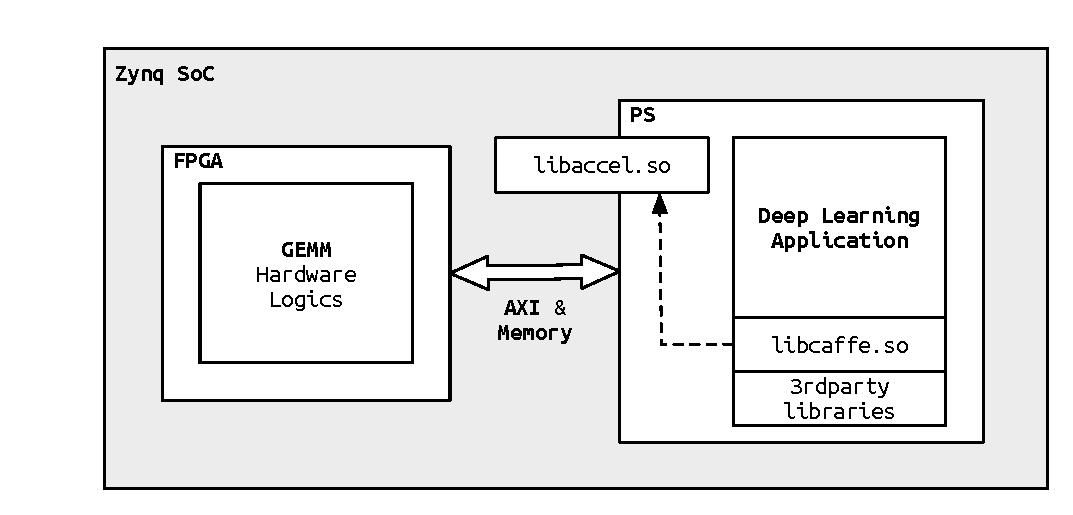
\includegraphics[width=0.9\textwidth]{assets/imgs/socaffe}
\caption{SoCaffe的系统架构}
\label{fig:socaffe}
\end{figure}

接下来分别介绍FPGA的加速器实现与ARM处理系统的实现工作。

\section{FPGA加速器实现}

基于FPGA实现的GEMM加速器是本研究的关键工作。本研究使用Vivado HLS工具设计并实现了基于固定大小的矩阵块之间的GEMM计算,并使用多种资源分配和调度策略进行优化;处理系统与FPGA之间的数据通路使用SDSoC工具提供的IP核实现;最后通过链接使得Caffe可以使用GEMM加速器进行计算。整个GEMM加速器基本使用了全部的FPGA硬件资源,相对于运行于CPU上的OpenBLAS库有5.45x倍速度提升,相应的测试结果在第四章详述。

\subsection{GEMM实现}

% GEMM算法特性的介绍
GEMM本身并不复杂,以传统的三重循环实现的矩阵乘法为基础就可以在CPU上实现。下面的算法中以矩阵$\mathbf{C}$的行、列为优先,假设每次迭代的坐标为$(i,j)$。每次迭代首先把$\beta \times \mathbf{C}(i,j)$作为累积变量$sum$的初值,进而遍历矩阵$\mathbf{A}$和$\mathbf{B}$的$i$行与$j$列(如果$\mathbf{A}$或$\mathbf{B}$需要转置则使用$i$列或$j$行,算法的5、6行使用了C语言的三元条件表达式表示转置条件),将$\mathbf{A}$与$\mathbf{B}$的对应元素和$\alpha$相乘并累加。最后把$sum$赋给$\mathbf{C}(i,j)$。


\begin{algorithm}
\caption{GEMM的原始三重循环算法}
\label{alg1}
\algsetup{indent=2em}
\begin{algorithmic}[1]
\FOR{$i=0$ \TO $M$}
  \FOR{$j=0$ \TO $N$}
    \STATE{$sum \leftarrow \beta \times \mathtt{C[i][j]}$}
    \FOR{$k=0$ \TO $K$}
      \STATE{$a \leftarrow \mathtt{(TA)\ ?\ A[i][k]\ :\ A[k][i]}$}
      \STATE{$b \leftarrow \mathtt{(TB)\ ?\ B[k][j]\ :\ B[j][k]}$}
      \STATE{$sum \leftarrow \alpha \times a \times b$} 
    \ENDFOR
    \STATE{$\mathtt{C[i][j]} \leftarrow sum$}
  \ENDFOR
\ENDFOR
\end{algorithmic}
\end{algorithm}


\subsubsection{GEMM分块矩阵算法}
% 分块的原理
如果要将该算法移植到FPGA上,首先需要对矩阵计算进行分块。FPGA上只有有限的硬件资源,而且在计算开始之前已经固定,所以不可能进行使用该算法在FPGA上计算任意大小的矩阵。所谓分块(tiling),是指将原先以矩阵元素为单元的遍历方式,改变为以固定大小的矩阵块为单元的遍历方式。分块矩阵算法的基本原理是分块矩阵乘法与分块矩阵转置的计算公式(如图3.2,3.3)。

\begin{figure}[!ht]
\[
\begin{pmatrix}
  A_{1,1} & A_{1,2} & \cdots & A_{1,k} \\
  A_{2,1} & A_{2,2} & \cdots & A_{2,k} \\
  \vdots  & \vdots  & \ddots & \vdots  \\
  A_{m,1} & A_{m,2} & \cdots & A_{m,k} 
\end{pmatrix}
\times
\begin{pmatrix}
  B_{1,1} & B_{1,2} & \cdots & B_{1,n} \\
  B_{2,1} & B_{2,2} & \cdots & B_{2,n} \\
  \vdots  & \vdots  & \ddots & \vdots  \\
  B_{k,1} & B_{k,2} & \cdots & B_{k,n} 
\end{pmatrix}
=
\begin{pmatrix}
  C_{1,1} & C_{1,2} & \cdots & C_{1,n} \\
  C_{2,1} & C_{2,2} & \cdots & C_{2,n} \\
  \vdots  & \vdots  & \ddots & \vdots  \\
  C_{m,1} & C_{m,2} & \cdots & C_{m,n} 
\end{pmatrix}
\]

\caption{分块矩阵的乘法运算}
\end{figure}
\begin{figure}[!ht]
\[
\begin{pmatrix}
  A_{1,1} & A_{1,2} & \cdots & A_{1,k} \\
  A_{2,1} & A_{2,2} & \cdots & A_{2,k} \\
  \vdots  & \vdots  & \ddots & \vdots  \\
  A_{m,1} & A_{m,2} & \cdots & A_{m,k} 
\end{pmatrix}^T
=
\begin{pmatrix}
  A_{1,1}^T & A_{2,1}^T & \cdots & A_{m,1}^T \\
  A_{1,2}^T & A_{2,2}^T & \cdots & A_{m,2}^T \\
  \vdots    & \vdots    & \ddots & \vdots    \\
  A_{1,k}^T & A_{2,k}^T & \cdots & A_{m,k}^T 
\end{pmatrix}
\]

\caption{分块矩阵的转置运算}
\end{figure}

上述公式中的矩阵元素都是矩阵块,每个矩阵中的矩阵块大小一致。$m$,$n$,$k$分别为按照块大小划分后的矩阵中块的个数。分块矩阵乘法运算的结果中,每个结果矩阵块都是由块之间的乘法和累加构成的:
$$\mathbf{C}_{i,j}=\sum_{t=0}^{k} \mathbf{A}_{i,t} \times \mathbf{B}_{t,j}$$

而分块矩阵转置运算的结果相当于先以矩阵块为单元进行转置,之后分别对每个矩阵块进行内部转置。

从上述两个公式出发便可以得到GEMM的分块矩阵算法。$BLK\_M$,$BLK\_N$,$BLK\_K$分别为矩阵的块尺寸参数。本算法的框架基本与GEMM原始算法类似,但是其中计算参数都是矩阵块而不是矩阵元素。

\begin{algorithm}
\caption{GEMM的分块矩阵算法}
\begin{algorithmic}[1]
\FOR{$bi = 0$ \TO $\lceil M/BLK\_M \rceil$}
  \FOR{$bj = 0$ \TO $\lceil N/BLK\_N \rceil$}
    \STATE{$\mathbf{S} \leftarrow \beta \times \mathbf{C}_{bi,bj}$}   
    \FOR{$bk = 0$ \TO $\lceil K/BLK\_K \rceil$}
      \STATE{$\mathbf{A}_b \leftarrow \mathbf{A}_{bi,bk}$ or transposed $\mathbf{A}_{bk,bi}^T$}
      \STATE{$\mathbf{B}_b \leftarrow \mathbf{B}_{bk,bj}$ or transposed $\mathbf{B}_{bj,bk}^T$}
      \STATE{$\mathbf{S} \leftarrow \alpha \times \mathbf{A}_b \times \mathbf{B}_b + \mathbf{S}$}
    \ENDFOR
    \STATE{$\mathbf{C}_{bi,bj} \leftarrow \mathbf{S}$}
  \ENDFOR
\ENDFOR
\end{algorithmic}
\end{algorithm}


接下来具体介绍如何把分块矩阵算法实现于FPGA上。

\subsubsection{硬件加速实现}\label{subsubsec:normal}

FPGA上主要加速的是GEMM分块矩阵算法的第7行,对两个固定大小的矩阵块求乘法并进行累加。因此,矩阵块的大小不能任意取值,主要受限于FPGA的硬件资源数量:越大的矩阵需要越多的板上计算资源和存储资源。此外,为了适配Caffe的接口,该算法主要针对单精度浮点数格式设计实现。最后,为了简化FPGA实现的接口,CPU端会分配几个固定大小的矩阵块用来保存传输到硬件的参数。

\begin{figure}[!ht]
\centering
\includegraphics[width=\textwidth]{assets/imgs/gemm}
\caption{GEMM的软硬件设计}
\end{figure}

图3.4是具体的硬件加速设计架构:左侧为FPGA可编程逻辑,右侧为处理系统,二者之间通过AXI总线通信。如图所示,每次计算会先从矩阵中复制矩阵块到专门划分的缓存区中,如果有需要转置则在复制过程中进行转置(如算法2的第5,6行)。之后,FPGA把缓存的矩阵块放入BRAM中,在每个迭代步都进行矩阵乘法运算中的点积操作。矩阵$\mathbf{C}$也被读入,和点积结果进行累加。FPGA上的数据写回到矩阵$\mathbf{R}$中,防止与对$\mathbf{C}$的访问冲突。当计算完成之后,处理系统使用矩阵$\mathbf{R}$的结果对内存中的矩阵$\mathbf{C}$进行更新,每次更新一个矩阵块大小的数据。

上述GEMM加速系统的设计的软件端代码可以很容易地实现,但是硬件端代码主要有两部分组成:将总线中的数据复制到BRAM,以及从BRAM中读取数据进行计算。硬件逻辑代码如代码\ref{lst:gemmaccel}和代码\ref{lst:gemmaccelkern}所示。
\begin{listing}[!ht]
\inputminted[
  mathescape, 
  linenos,
  numbersep=5pt,
  breaklines=true,
  fontsize=\footnotesize]{c}{assets/codes/hls.c}

\caption{\texttt{gemm\_accel}函数的定义(未优化)}
\label{lst:gemmaccel}
\end{listing}

\begin{listing}[!ht]
\input{assets/codes/hlskern.tex}
\caption{\texttt{gemm\_accel\_kernel}函数的定义(未优化)}
\label{lst:gemmaccelkern}
\end{listing}

% 简单介绍代码的情况
这两份代码都默认矩阵块的大小必须完全相同,这是一种简化,在实际实现的代码中尺寸可以不一致。\texttt{gemm\_accel}是被指定为要被HLS生成硬件的函数,因此\texttt{Ab},\texttt{Bb}与\texttt{Cb}都会被实现为FPGA上的BRAM\footnote{有的时候HLS工具也会用LUT来生成存储,选择BRAM还是LUT可以在程序中显式指定},\texttt{gemm\_accel}所调用的\texttt{gemm\_accel\_kernel}中的计算过程也会被实现为硬件逻辑。

\subsubsection{基本优化技巧}
两个函数中出现的循环一般会被实现为硬件逐步迭代进行的计算,但因为在代码中使用HLS的流水线预编译指令(pipeline),因此循环的迭代步之间可以同时执行:上一步迭代的计算与这一步迭代的BRAM读取不冲突,可以并行。流水线化是实现高效硬件逻辑的关键步骤,在Vivado HLS工具中,流水线化与循环控制流密切相关,被流水线化的循环内部的嵌套循环会被默认进行循环展开(Loop Unrolling)。同时,初始化间隔(Initialization Interval,简称II)指的是流水线需要几个时钟周期才能进行初始化,当II=1时流水线化达到最佳水平。II=1的结果主要因为对A和B的数组划分(Array partition):对A与B的访问可以同时通过多个端口进行,这样流水线便不会阻塞。

\begin{table}[!ht]
	\centering	
	\begin{tabular}{ | l | l | l | l | l |}
		\hline
		BRAM\_18K (\%) & DSP48E (\%) & FF (\%) & LUT (\%) & Latency (cycles) \\ \hline
		23 & 72 & 18 & 46 & 2352 \\ \hline
	\end{tabular}
	\caption{当前代码的HLS结果,包含资源占用率与预测延迟}
	\label{table:gemmorig}
\end{table}

对上述代码进行高层次综合可以得到一份简单的报告,进而可以分析得到当前代码的理论效率与资源占用情况。表\ref{table:gemmorig}是针对上述算法综合的$\mathtt{Dim}=32$的GEMM计算硬件资源占用。

% 性能预测与高层次综合报告
\subsection{GEMM性能分析与预测}

% 前提假设
本节从GEMM算法的特性出发,找出性能与GEMM分块算法中的块大小之间的数学关系。性能指标的单位为GFLOPS(Giga floating-point operations per second,每秒1G次浮点运算操作个数)。由于GEMM分块算法有多种分块方式,为了简便起见本节中使用正方形划分的分块方式,即从矩阵$\mathbf{A}$,$\mathbf{B}$,$\mathbf{C}$划分出的任意块$\mathbf{A_{ik}}$,$\mathbf{B_{jk}}$与$\mathbf{C_{ij}}$都是正方形。此外,本节性能分析只涉及FPGA硬件逻辑的计算时间,数据传输延迟暂不考虑。

% FPGA的性能预测概论
理论上,FPGA的运行时间($time_{HW}$)延迟($latency$,单位为时钟周期数)和时钟频率($freq$,单位为MHz)相关:

\begin{equation}\label{eq:timelatency}
time_{HW}=\frac{latency}{freq}
\end{equation}
% $$\mathtt{time} = \mathtt{latency} \times 1 / \mathtt{frequency} = 2352 / (143 \times 10^{6}) s = 1.64 s$$

% 延迟大小与GEMM块大小的关系
延迟的大小与GEMM使用的矩阵块大小密切相关。矩阵块大小由三个参数决定:$Dim_M$,$Dim_N$,$Dim_K$\footnote{$M$,$N$,$K$的语义与描述矩阵乘法的场景中使用的语义一致,即$Dim_M$为矩阵块$\mathbf{A_{ij}}$的高,$Dim_K$为其宽。其余可以类推得到。}。
原始实现(如\ref{subsubsec:normal}节所示)中延迟由两个子过程决定,分别为BRAM复制与GEMM计算。
% BRAM复制与GEMM块大小的关系
BRAM复制过程包含三个独立的、流水线化的循环,总延迟(\(\mathit{L_{BRAM}}\))等于三个循环的延迟之和。
假设初始化间隔已经达到目标1,则流水线化的循环延迟约等于循环体的延迟\footnote{\(\mathbf{A}\)矩阵块的BRAM复制循环与其他循环不同,延迟主要取决于与\(\alpha\)的乘法计算延迟,因为乘法比赋值更慢}加上循环周期数,因此:
\begin{equation}\label{eq:bramcopylatency}
\begin{aligned}
\mathit{L_{BRAM}}
& = \mathit{L_{AMultLoop}+L_{BCopyLoop}+L_{CCopyLoop}} \\
& = \mathit{Dim_M\times Dim_K + L_{mult}} 
  + \mathit{Dim_N\times Dim_K + L_{copy}} \\
& + \mathit{Dim_M\times Dim_N + L_{copy}} \\
& = \mathit{S_A + S_B + S_C + 2L_{copy} + L_{mult}} 
\end{aligned}
\end{equation}
%对于固定大小矩阵块的GEMM计算而言,一次运算共进行$\mathtt{Dim}^3\times2+\mathtt{Dim}^2+\mathtt{Dim}^2\times 2 = 2\mathtt{Dim}^3+3\mathtt{Dim}^2$次浮点数运算。因此理论上GFLOPS(每秒G次浮点数运算)的结果为:
%$$\mathtt{GFLOPS} = (2\mathtt{Dim}^3+3\mathtt{Dim}^2)/\mathtt{time} = 4.17$$
即BRAM复制过程的延迟等于三个矩阵块的面积和与两个复制的延迟(\(\mathit{L_{copy}}\))、一个乘法运算的延迟(\(\mathit{L_{mult}}\))的和。
% 乘法计算与GEMM块大小的关系
GEMM计算延迟(\(\mathit{L_{comp}}\))取决于流水线化的GEMM三重循环计算,由于其中第二层循环被流水线化,这部分的总延迟等于前两层的循环周期数加上第三层循环完全展开后的点积计算延迟(\(\mathit{L_{prod}}\)):
\begin{equation}\label{eq:complatency}
\begin{aligned}
\mathit{L_{comp}}
& = \mathit{Dim_M \times Dim_N + L_{prod}} \\
& = \mathit{S_C + Dim_K \times L_{add} + L_{others}}
\end{aligned}
\end{equation}
简单对数据流进行分析可以发现,由于点积运算中包含存在依赖的求和运算,且这部分的延迟与\(\mathit{Dim_K}\)成正比
\footnote{根据\cite{ug902}第183页,对于浮点数格式的加法,为了防止出现精度问题,不会使用平衡过的加法树(Adder Tree),因此延迟与\(Dim_K\)的关系是线性而不是对数的。}
,因此GEMM计算延迟与\(\mathit{Dim_K}\)相关。

% 总延迟
综上,假定矩阵块面积的大小是主要决定因素(其他延迟变量的值暂且忽略不计),且令\(\mathit{Dim}\)为最大矩阵块尺寸,则综合公式\ref{eq:bramcopylatency}与\ref{eq:complatency},得到总延迟的表达式为:
\begin{equation}\label{eq:latency}
\begin{aligned}
\mathit{latency} 
& = \mathit{L_{BRAM}} + \mathit{L_{comp}} \\
& \approx \mathit{S_A + S_B + 2S_C} \leq 4Dim^2
\end{aligned}
\end{equation}
即总延迟的大小的上界为\(\mathit{4Dim^2}\)。

% 总浮点数操作数
GEMM的浮点数操作数总数(\(\mathit{FLOP}\))也取决与矩阵块尺寸。从GEMM的公式出发\ref{eq:gemm},得到(公式\ref{eq:flop}中的下标为特定的运算步,\(\mathit{Dim}\)依然为矩阵块尺寸中的最大值):
\begin{equation}\label{eq:flop}
\begin{aligned}
\mathit{FLOP} 
& = \mathit{FLOP_{\mathbf{AB}}} 
  + \mathit{FLOP_{\alpha\mathbf{AB}}}
  + \mathit{FLOP_{\beta\mathbf{C}}}
  + \mathit{FLOP_{\alpha\mathbf{AB}+\beta\mathbf{C}}} \\
& = \mathit{2 Dim_M\times Dim_N\times Dim_K + Dim_M \times Dim_N} \\
& + \mathit{Dim_M \times Dim_N + Dim_M \times Dim_K} \\
& = \mathit{2 S_C \times Dim_K + 3 S_C} \\
& \leq \mathit{2 Dim^3 + 3 Dim^2}
\end{aligned}
\end{equation}

% GFLOPS
综合公式\ref{eq:latency}与\ref{eq:flop}可得:
\begin{equation}\label{eq:gflops}
\begin{aligned}
\mathit{GFLOPS}
& = \mathit{\frac{FLOP}{latency} \times frequency \times 10^{-9}} \\
& = \mathit{\frac{2 Dim^3 + 3 Dim ^ 2}{4 Dim^2}\times frequency \times 10^{-9}} \\
& = \mathit{\frac{2 Dim + 3}{4} \times frequency \times 10^{-9}}
\end{aligned}
\end{equation}
随$\mathit{Dim}$的增加,$\mathit{GFLOPS}$上升。

% 结论
综上,GEMM计算的硬件性能与使用的矩阵块的最大尺寸成正比,因而优化的目标应为最大化GEMM中使用的矩阵块大小。矩阵块大小的上限取决于FPGA上各类资源的总量,和GEMM硬件设计使用各类资源的方式。下一节具体阐述如何通过修改HLS生成硬件设计的方式来优化GEMM的算法效率。

\subsection{GEMM优化}\label{subsec:gemmopt}

% 引言 介绍前文中提到的算法和设计的问题
一个硬件设计应该充分使用FPGA的各类资源。根据表\ref{table:gemmorig},该设计使用了大量的DSP,而其他资源的利用率都很有限。实际上经过测试,当$\mathtt{Dim}=48$时对DSP的使用几乎达到最高,无法继续扩大$\mathtt{Dim}$的取值了。一种想法是将使用DSP资源的计算用LUT等资源实现。此外,通过牺牲精度、使用更小的数据类型来降低每个操作所占用的资源,进而提高矩阵块的大小也是一种关键优化策略。本节使用固定小数点数据类型(fixed-point data type)作为优化目标。此外,通过使用不规则的矩阵块也可以提高$\mathtt{GFLOPS}$。针对数据传输和任务执行模型的优化在本节中也会涉及。

% 优化硬件资源分配
\subsubsection{优化硬件资源分配}

为了在不增加延迟的基础上降低DSP的使用,本研究将部分计算强制使用非DSP资源实现。默认的浮点数乘法与加法运算都需要同时占据DSP与LUT来实现其功能。此时,如果使用Vivado HLS的resource预编译指令,就可以指定某个参数一定要使用某一种资源来实现。对于包含循环的设计而言,一个操作往往会在多次迭代中频繁使用。对于这种情况,如果将该运算完全用LUT或其他资源实现,可能会造成DSP的使用与LUT的使用再次失衡,甚至会导致LUT的使用超出系统上限。综上,本研究提出一种有效地优化硬件资源分配,均衡不同资源使用的方法:通过手动指定使用DSP的操作的迭代范围,来最大化对硬件资源的利用(如代码\ref{lst:gemmaccelkernopt}所示)。

\begin{listing}[!ht]
\inputminted[
  mathescape, 
  linenos,
  numbersep=5pt,
  breaklines=true,
  fontsize=\footnotesize]{c}{assets/codes/hlskern-opt.c}

\caption{\texttt{gemm\_accel\_kernel}函数片段:优化硬件资源分配}
\label{lst:gemmaccelkernopt}
\end{listing}

\texttt{LUT\_RANGE}与\texttt{DSP\_RANGE}给出了使用的加法操作应该用什么方式实现的范围:HLS指令的参数\texttt{FAddSub\_nodsp}是完全不用DSP实现浮点数加法,\texttt{FAddSub\_fulldsp}则全部使用DSP实现。使用该策略最终可以在FPGA上生成$\mathtt{Dim}=64$的GEMM计算单元。相应性能测试在第四章中详述。

% 大小不等的矩阵块
\subsubsection{优化矩阵块形状}
之前的假定是矩阵块的大小尺寸必须完全一致,主要是为了在数据复制的步骤中使用一套循环逻辑来降低延迟。但如果将条件放松一些,当$M$与$N$对应的块尺寸相等,$K$对应的块尺寸相异时,循环逻辑依然可以保持不变,只需要增加循环内部的条件判断即可。允许大小不等的矩阵块的优点在可以更精细地调整硬件资源的使用。BRAM的使用由三个块尺寸同时决定,而计算单元只是由$K$对应的块尺寸决定。因此在DSP和LUT的资源达到上限的时候,还可以通过增加$M$与$N$对应的块尺寸来增大BRAM的资源占用,从而提高FPGA每次运算的运算量。

\begin{listing}[!ht]
\input{assets/codes/hlskern-irr.tex}
\caption{\texttt{gemm\_accel}函数:优化矩阵块形状}
\label{lst:gemmaccelopt}
\end{listing}

% 使用half
\subsubsection{优化数据类型}
尽管上述几种优化策略已经能在FPGA上部署很大的矩阵块,执行很快的GEMM算法了。但是针对某些特殊的场景,比如要求实时性的计算时,之前的优化结果尚并不如人意。在这些场合中,对速度的要求高过对精确度的要求,因此可以使用更低精度的数据类型来降低平均每次计算所用到的资源,进而增加板上部署的矩阵块的大小。

\begin{figure}[!ht]
\centering
\includegraphics[width=0.4\textwidth]{assets/imgs/half}
\caption{IEEE半精度浮点数的格式定义}
\end{figure}

HLS提供了半精度浮点数(Half-precision floating point)的支持,其格式包含1个符号位,5个指数位和10个尾数位,共16位。半精度浮点数已经广泛地应用于计算机图形学等领域了。这里的优化实现方法只是将板上BRAM存储的矩阵块都用半精度浮点数声明,不改变输入参数的类型与处理系统中声明的数据类型。在FPGA的计算内核中使用半精度浮点数进行强制类型转换。

经过测试,使用半精度浮点数的GEMM算法可以使用最高达到$Dim=96$的矩阵块。此外,由于半精度浮点数运算使用很少的资源,因此可以令$K$对应的块尺寸变得很大,以充分利用板上的计算资源。

综上,GEMM的优化目标是尽可能地利用FPGA的资源,以部署更大的矩阵块来提高计算效率。使用了这一系列优化方式之后,GEMM自身相对于纯CPU的实现已经取得了很大的加速比。下一节具体描述如何令Caffe运行于Zynq SoC上,并与GEMM加速器相结合。

\section{ARM系统实现}

SoCaffe在处理系统上的工作(如图\ref{fig:socaffe})主要分为三个部分:编译与优化使用硬件加速库、交叉编译Caffe与其他第三方库、生成SD卡文件包。本节的工作主要依赖SDSoC工具,使用其提供的IP核、代码生成来构建与FPGA加速器的通信机制,ARM GNU工具链构建动态链接库和交叉编译,bootgen等工具生成包含比特流的Linux系统镜像等等。

% 链接加速器库
\subsection{构建与使用硬件加速库}

尽管在Caffe中使用GEMM加速库只用调用封装好的硬件加速器入口函数即可,但还有些问题需要考虑。首先,GEMM加速器并不适合全部形状的矩阵参数:当矩阵尺寸比较小时,使用GEMM加速器甚至比软件版本慢很多,主要原因是GEMM加速器的额外开销与计算对小尺寸矩阵计算时间而言是显著的。其次,在执行GEMM硬件加速函数的同时,CPU也应该利用起来,进行一些内存分配和复制等等简单操作,这就要求对GEMM硬件函数的调用代码需要异步执行。最后,GEMM硬件加速库与一般软件库不同,其中包含了一个硬件的比特流,选择何时加载、如何加载比特流也是需要考虑的问题。接下来会逐一讨论如何构建与使用GEMM硬件加速库。

\subsubsection{PS-PL接口生成}
调用GEMM加速器函数时,会以处理系统分配好的内存地址作为参数,SDSoC主要根据参数对应的内存块的分配方式来确定生成什么样的接口。如果内存块是以\texttt{malloc}分配生成的,则SDSoC使用Scatter-Gatter类型的接口访问内存中的数据。如果内存块以\texttt{sds\_alloc}分配,则SDSoC可以认识到该内存块是地址连续的,因此会使用顺序访问的接口(比如AXIDMA\_SIMPLE)。除此以外,如果不需要保证缓存的数据一致性,可以指定SDSoC生成使用AFI端口的高速访问数据通路,否则SDSoC会自动使用ACP端口。

\subsubsection{调用方式与条件}

在进行GEMM计算的同时,CPU端往往处于空闲状态。如果此时可以进行一些比较耗时的操作,比如复制数据到矩阵块缓冲区等等,那么系统性能可以得到不错的提升。SDSoC提供了预编译指令\texttt{async <ID>},用来标识硬件函数需要被异步调用;同时也提供了\texttt{wait <ID>}指令来指定等待硬件函数完成的时间点;其中\texttt{<ID>}用来对异步调用任务进行标记。这种异步机制本质上而言构建了FPGA与CPU之间的流水线,提高了系统的并行度。

\begin{listing}[!ht]
\input{assets/codes/caffegemm.tex}
\caption{\texttt{caffe\_cpu\_gemm}函数}
\label{lst:caffegemm}
\end{listing}

正如本节序言所述,GEMM加速器是针对固定大小的矩阵块实现的,因此无法根据输入矩阵的形状进行调整。尤其是当输入矩阵形状非常不规律时,比如一条边很短(~10)而另一些边很长(>1000)时,使用GEMM加速器会带来非常大的性能损耗。本研究使用一种简单条件来判断是否应该执行GEMM:只有当输入矩阵的三个尺寸都大于128时才调用GEMM加速器(如代码\ref{lst:caffegemm}所示,其中当定义了\texttt{SDS}时才会编译\texttt{gemm\_sds}接口),否则使用CPU端的BLAS库。根据测试结果,这种启发式的策略产生了不错的效果,Caffe的性能基本不受矩阵形状的影响了。

\subsubsection{链接库生成}

传统的Zynq SoC应用开发在完成硬件函数的设计之后,是无法使用类似于软件方式调用该硬件逻辑的:必须要通过配置AXI总线的数据并传输数据才能执行硬件逻辑。但使用SDSoC进行开发时却可以直接调用硬件函数,究其原因,主要是因为SDSoC在编译过程中对原始的硬件函数进行了封装,并将封装后的版本替换了原始的函数调用。封装的函数包含了额外的数据准备,信号传输与等待命令完成等一系列过程。正因为如此,SDSoC可以为FPGA硬件逻辑自动构造出一个软件动态链接库。

但硬件逻辑的比特流却不包含在动态链接库中,而是放在一个独立的数据文件中。比特流文件可以在系统引导的过程中加载,也可以在系统运行过程使用\texttt{xdevcfg}设备动态配置。

% 交叉编译
\subsection{交叉编译}

所谓交叉编译,指的是一种编译出来的程序是运行在其他环境中的编译过程。SDSoC中提供的ARM GNU工具链就是在x86环境中交叉编译出ARM环境中可执行代码的交叉编译工具。使用该工具链编译GEMM硬件加速库,以及Caffe本身都很简便,但是涉及到Caffe的第三方库依赖便会遇到很多问题。针对第三方库的交叉编译主要有三种策略:

\begin{enumerate}
\item 直接修改环境变量中的\texttt{CC},\texttt{LD}等为ARM GNU工具链中对应的工具,可以用来处理比较简单的库的编译;
\item 使用第三方库提供的配置方案进行交叉编译配置:大部分第三方库都会使用configure、CMake等工具生成\texttt{Makefile},以方便交叉编译; OpenBLAS在编译工具链的配置之外也会要求指定对应系统架构的名称,进而可以充分优化性能。
\item 其他:有的第三方库完全不支持交叉编译,主要原因是编译过程需要得到编译结果测试的反馈。比如HDF5在编译的过程中,会调用编译出来的程序来生成与目标系统相关的代码,处理起来非常麻烦。
\end{enumerate}

因为第三方库的交叉编译标准不一,而且目标环境相对固定,因此本研究提供一套已经编译好的第三方动态链接库供SoCaffe使用,不需要重复编译,直接链接即可运行。

% 其他细节
\subsection{系统生成}

系统生成过程需要得到最终的、可用的SoCaffe系统,其中要包含编译好的动态链接库,FPGA比特流,以及其他工具等等。本研究按照如下流程构建SoCaffe系统:

\begin{enumerate}
\item 编译硬件加速器动态链接库(\texttt{libaccel.so}),生成包含FPGA比特流的SD卡与相应的引导文件;
\item 编译Caffe链接库(\texttt{libcaffe.so}),并链接第三方库函数和硬件加速器函数;
\item 编译使用SoCaffe环境的代码,比如各种基于Caffe的深度学习应用等等;
\item 将所有生成的链接库,可执行程序复制到第一步生成的SD卡目录中,进而复制到Zynq SoC使用的SD卡;
\item 启动系统,将链接库复制到系统库目录下(\texttt{/lib}),运行需要执行的程序;
\end{enumerate}

\section{总结}

(暂无)